\documentclass[a4paper,11pt]{article}
\usepackage[osf]{mathpazo}
\usepackage{ms}
\usepackage[]{natbib}
\raggedright

\newcommand{\datastorr}{\texttt{datastorr}}
\newcommand{\smurl}[1]{{\footnotesize\url{#1}}}
\newcommand{\ghsmurl}[1]{{\footnotesize\href{https://github.com/#1}{#1}}}

\usepackage{graphicx}

\title{Versioned data: why it is needed and how it can be achieved (easily and cheaply)}
\author{Richard G. FitzJohn$^1$, Daniel S. Falster$^2$,\\ Matthew
  W. Pennell$^3$, and William K. Cornwell$^{2,*}$}
\affiliation{
$^1$ Imperial College, London, United Kingdom\\
$^2$ Evolution \& Ecology Research Centre, School of Biological, Earth and Environmental Sciences,\\
University of New South Wales, Sydney, NSW 2052, Australia\\
$^3$ Department of Zoology and Biodiversity Research Centre,\\
University of British Columbia, Vancouver, B.C. V6T 1Z4 Canada\\
$^*$ Corresponding author: w.cornwell@unsw.edu.au\\
}
\date{}

\bibliographystyle{mee}

\usepackage[title,titletoc,toc]{appendix}

\mstype{Article Note}
\runninghead{Versioned Data Delivery}
\keywords{Data sharing, Version control, Semantic versioning, Meta-analysis}

\begin{document}
\mstitlepage
\noindent
\parindent=1.5em
\addtolength{\parskip}{.3em}
\doublespacing
\linenumbers


% For Analyses and Articles, the main text (excluding abstract, Methods, references and figure legends) is approximately 3,000 words. The abstract is typically 100-170 words, unreferenced. An Introduction is followed by sections headed Results, Discussion, Methods. The Methods and Results should be divided by topical subheadings; the Discussion does not contain subheadings. The Methods should be followed by References, Data Citations (optional), Acknowledgements and a Competing interests statement. A Data Citation section should be included when externally hosted datasets are referred to in the work and each can be cited formally with a unique, stable identifier and repository name.



\section{Summary}

The sharing and re-use of data has become a cornerstone of modern science.  To help this process, numerous linked tools have been developed to allow quick and easy data sharing:    a data file for a particular analysis can be quickly uploaded, given a digital identifier, and shared.  Thus far, however, this framework does not account for on-going scientific progress: for many important problems, epitomised by problems that lead to one or more meta-analyses, datasets will continue to grow with time---more data points will be added, and new and more useful data structures will be created.  Essentially this means that datasets, like science in general, progress with time.  We suggest that many different datasets would be more useful if organized as a series of versions, with a simple naming system to allow users to perceive the type of change between versions.  In this article, we argue that adopting the paradigm and processes for versioned data, analogous to software versioning, would be useful for both data curators and users of even small-to-medium sized datasets. We introduce a system called Versioned Data Delivery (VDD) and present tools for creating, archiving, and distributing versioned data easily, quickly, and cheaply. These new tools allow for individual research groups to shift from a static model of data curation to a dynamic and versioned model that naturally matches the scientific process.

\section{Introduction}

As is evidenced in the advent of this journal, publication of quality datasets is now considered a first-class scientific product. Increasingly, funding bodies, publishers, and scientific social norms are recognizing the value of sharing data, including as standalone products without any accompanying analyses \cite[e.g.][]{Whitlock-2011,Fairbairn-2011,Piwowar-2011,VanNoorden-2013,Gibney-2013,Editorial-2014}. Datasets are now routinely archived as part of the publishing process. Moreover, increasing numbers of standalone ``Data papers'' (or descriptors) have been appearing in standard domain-level journals, as well as specialised data journals, like \emph{Scientific Data}. Yet, while the last decade has witnessed a rapid and exciting change in attitudes towards data sharing and publishing, the scientific community is still grappling with how to effectively disseminate and manage open-source datasets \cite{Whitlock-2011, Goodman-2014, Lowndes-2017,Perkel-2016,VanNoorden-2013, Kratz-2015}. In particular, the current data publishing model has not yet embraced the idea that many  datasets are designed to answer scientific questions that extend beyond the scope of a single empirical paper.  These datasets are constantly evolving, i.e. never "finished", and may be the subject of repeated analysis or meta-analysis.

Many, and perhaps most, of the datasets published in this journal are likely to be living entities, meaning the state-of-the-art version of the dataset will changes through time. Typical changes may involve: the addition of new data, improving the quality of existing data, better linked to external databases, or re-structuring of the database content to be able to address new questions. For example a dataset on a biological organisms might be expanded through the addition of new records or improved through the correction of spelling mistakes in taxonomic names. As research around a data product grows, there might be many such additions. Ideally, any changes to a dataset would become immediately available to any interested parties, while -- to ensure reproducibility -- past versions of the dataset would remain accessible.

Unfortunately, current models for publishing datasets do not immediately solve the issue of how to distribute successive versions of a dataset in an effective and scalable manner. The most common current working model for publishing scientific datasets is to archive them in a variety of open-source data repositories -- such as \texttt{Dryad}, \texttt{Figshare}, or \texttt{Zenodo} -- where the data is attributed a Digital Object Identifier (\textsc{doi}). Once published, the datasets are immutable. That means that most published datasets exist as a singular snapshot of the dataset, taken at the time the data descriptor was published. While it might only require a small amount of work to update the dataset, if there is no way to distribute the updated dataset, then that work has to be re-done by every user of that dataset. Moreover, those required changes add steps between the canonical dataset and any analysis using it, making reproducibility of the new analysis more difficult than it needs to be.

Many research groups internally solve the issue of versioning data in a variety of suboptimal ways. A common solution is to email around the latest versions with version numbers appended to the filename. Another approach is to repeat corrections or updates that have been made elsewhere. This practice is both inefficient and a barrier to reproducibility, as the dataset used in a publication may differ to the version previously made available on-line. There is therefore a strong need for an easy way to distribute changes to a dataset after its initial publication to potential users, along with notes on what has changed and why since the previous version.

In this article we i) introduce the concept of Versioned Data Delivery (\textsc{vdd}); ii) outline how emerging technologies in data science (Table \ref{tab:technologies}) can be used to help researchers maintain, distribute, and access small-to-medium sized datasets; and iii) introduce a new \textsc{R} package called \texttt{datastorr}, a proof-of-concept implementation of a \textsc{vdd} system. The issue of updating and expanding published data has been partly addressed in large centralised repositories like genetic sequences (\texttt{GenBank}) or species location data (\texttt{GBIF}), where new data can be added and there exist abilities to correct errors in existing records (e.g. by adding multiple version of a genetic sequence). Yet, such large centralised repositories require a level of infrastructure that is beyond most research groups, or even countries (Table \ref{tab:sql_v_versioneddata}). Our focus here is on the wide range of datasets not covered by these repositories, such as those appearing in this journal. In most of these cases, the data collected will not be ``big'' but rather small-to-medium sized. Such data support important research projects on particular scientific questions, but are not in most cases general enough to warrant custom infrastructure. Further, while we emphasize particular technologies in our implementation, the principles are general and could easily be ported to other platforms. Likewise, while the examples cited here come from our own research areas the issues we have identified and the solutions we have put forward are relevant to nearly all data-oriented scientific domains.


% I think that this model is actually ok; for data archiving where the
% data are a record of what was used in the paper, a single immutable
% data set makes sense.  It just doesn't extend to things where the
% research output *is* the dataset.  So this is more a case of
% pointing out that this model does not apply well to all sorts of
% data - given how successful the archive-at-publication model has
% been at getting data out of people's drawers I don't think we should
% complain that it doesn't do something that it does not need to do.

% A particular issue with the static
% model is that data releases are mostly triggered by publication of academic
% papers. But for a living dataset, there may be multiple releases made in
% between papers. This is particularly the case with the discovery of small
% errors.
% % OK, here again; it's not so much medium-sized as *living*.  The
% % issues in practically doing the versioning are more acute when the
% % data are bigger than small, that's all.
% For any living dataset that is put to reuse, errors will
% inevitably be found, and there needs to be some easy  way to correct them and
% distribute the updated dataset.

% To overcome the limitations of static datasets, many research groups have
% setup dedicated webservers to host and distribute data (Table 1)\citep[e.g.][]{Madin-2016}. In these systems,
% datasets areas maintained in a structured database, such as SQL, and a custom front
% end to this database must be written.
% When designed well, such systems are very useful for updating or adding to a
% dataset. However, the infrastructure investment (designing maintaining, and
% hosting the database) is overkill for most projects and is a very
% substantial barrier to entry. Furthermore, the system requires ongoing funds to maintain it, making it often unsustainable for many research groups. Moreover, the existence of a live webserver,
% does not in itself guarantee ongoing access to different versions of a
% dataset.


\section{A lightweight, cheap, and scalable workflow for delivering versioned data}

% I really like the focus on "release".  It's a happy coincidence that
% it's what github uses in the interface.

In brief, the workflow we present, which we call Versioned Data Delivery (\textsc{vdd}), borrows best-practices for software development \cite{Perez-Riverol-2016} and applies them to the challenge of maintaining and distributing versioned data. Software developers maintain a core set of code which produces a binary executable file that can be installed on a users local computer. With a \textsc{vdd} system, data developers similarly maintain a core set of files (the ``code''), which produce an organised dataset that can be ``installed'' on a user's local computer. In either the development of software or data, successive versions are released over time (called ``releases''). The similarity in workflow between software and data then allows us to deploy the same technological platforms that are used in software development, for the development and distribution of data. Importantly, our \textsc{vdd} systems uses well-established tools, ensuring high-level performance and stability.

The core technologies used are summarised in Table \ref{tab:technologies} and described further below.

\subsection{Version control}

% You could
% talk about 'git' (referencing Ram-2013) and say "on the face of it,
% versioning tools like git appear to provide the ideal interface for
% versioning data".  Then talk about how git is designed for code and
% breaks down as the data involved exceed a few 10s to hundreds of MB.
% After that, we can say that the aim is not to support truely "Big"
% data because research groups capable of generating such data
% probably have the wherewithall to look after it.  I know you bring
% it up below, but I think it would go better here...

% With suggested edits, some of this moves up.
Version control, primarily an open-source variety called \texttt{git}, has become ubiquitous in software development. In practice, version control tracks line-by-line changes in text files and creates and maintains a history of those changes. Increasingly version control has been applied to scientific code and data management, especially for small-to-medium sized datasets \citep{Ram-2013, Perkel-2016}. \texttt{git} is attractive for data management because it tracks all changes in monitored files. This history is visible to anyone interacting with the repository. It also allows users to annotate changes (`commits') with informative messages detailing the rationale for those changes.
  
% So, git doesn't actually work this way, though everyone seems to
% think that it does.  Git stores *content* and then later tries to
% de-duplicate it.  It then displays changes as line-by-line diffs
% (but you can change this to display the changes other ways; see
% --color-words --ignore-all-space for example.  The problem is that
% the algorithms that git uses are optimised for typical sizes of code
% and not for data.  Small data is actually totally fine to store with
% git.  The other issue that turns up is if the files are _binary_
% then an arbitrarily small change in the underlying data can result
% in an arbitrarily large change in the binary representation, which
% prevents deduplication.
%
% Git-LFS tries to step around this by storing large files separately
% from git's general machinery.  Git-annex did the same.  But they
% suffer from some of the other issues with git which are that it's a
% bit of a pain for (especially novice) users to do nontrivial things
% with.  I _always_ have to look up how to compare two versions across
% branches.  And there's no simple way of loading in two versions of
% the data into R without ending up with two working copies or doing
% some nasty "git show" call.
Because \texttt{git} was built for tracking changes in code, there are aspects of how it behaves that are not natural to apply to  data \cite{Perkel-2016}.  For example, because it tracks changes line-by-line rather than cell-by-cell, there are inefficiencies in how the software stores the changes.
% Dan Noble: I think this is a pragmatic view, but I would have a tendency not to discuss how the tools you can use for a VDD approach are likely to be "replaced in the near future”. Of course, things change, but this will not entice the people you want the paper to appeal to to adopt this sort of approach. From my experience, some of the resistance to adopting this stuff comes from programs or repositories being “replaced” at such a high rate. They just don’t feel like its worth doing.
There is rapid current work on new implementations which will be faster computationally, smaller in file size, flexible with respect to data structures, and thus allow for larger datasets to be versioned efficiently\citep{Fli, Dat}.
% Add CKAN here?
That said, the workflow we describe here currently works well with \texttt{git} and should work even more quickly with its future replacement.


\subsection{`Semantic' versioning}

% WKC: this is back to our main point

To fully realize the benefits of a versioned data, the \textsc{vdd} system needs to be communicated to the user.  Crucially a user should be immediately aware of the relationship among versions.  Software development has dealt with a very similar problem, and we suggest there is benefit in adopting the notation from that field.  Specifically, we suggest applying the theory of ``semantic versioning'' developed for software distribution. This system uses (the potentially familiar) notation of form ``1.0.0'' for successive versions (Fig \ref{fig:semantic}). As has been noted (REFS), labelling of data versions presents a similar problem to the labelling of software releases: signalling to users the types of change that has occurred between successive versions. Applying semantic versioning to data, a change from 1.0.0 to 1.0.1 implies tiny changes, for example a minor error correction. A change from 1.0.0 to 1.1.0 implies a substantial enhancement, for example adding a new study to a meta-analysis dataset (while otherwise maintaining the same dataset structure). A change from 1.0.0 to 2.0.0 implies a very major revision, for example improving the entire structure of the dataset and adding new columns.
% I think that major version increments could still be looked at as
% _breaking_ changes as often as large additions of data.  Changing
% column names, removing columns, changing the structure of linked
% tables etc.


\subsection{Distributing data to different user needs}

At current there are two classes of data users: those that  interact with the data via point and click downloading and those that use code-based interaction.  The system we describe allows for both types (Figure \ref{fig:technology_stack} and Table \ref{tab:user_requirements}).  \texttt{GitHub} has a feature called ``releases'' in which specific commits can be turned into a version for distribution (with associated version number).  Those releases can be downloaded directly by users via point-and-click, or accessed via the \texttt{GitHub} \textsc{api}.
% I have no idea what this next sentence means.
Releases can also be embedded into any kind of website that allows the data curator to facilitate discovery by more users and to provide context.  Releases can also be linked to digital object identifiers and code-based users via for example an \textsc{R} package.

\subsection{\texttt{datastorr} and dataset-specific \texttt{R} packages}

A point-and-click workflow may create barriers for reproducibility \cite{Wilson-2014,Lowndes-2017}. Ideally, users should be able to access all versions of the database programmatically. Code to access the \texttt{GitHub} releases could be written individually by each user, but this creates an unnecessary technological hurdle for reproducibility.  To make access via code as easy as possible for users, we offer a novel implementation of a \textsc{vdd} system. We have written an \textsc{R} package, \texttt{datastorr} (\smurl{github.com/richfitz/datastorr}), that a) interacts with the \texttt{GitHub} \textsc{api} to pull down versions of the dataset; and b) constructs the shell of a second, database specific \textsc{R} package, which can be used to access versions of the dataset. Using this system, a researcher can create and distribute a \textsc{R} package that facilitates access to their data with (very) minimal computational skills. We have focussed on the \texttt{R} platform \cite{R-2017} as one of the most prominent platforms for data analysis.

For example, \texttt{datastorr} was used to build the package \texttt{baad.data} (\smurl{github.com/traitecoevo/baad.data}), which is an interface to the Biomass and Allometry Database (\textsc{BAAD}) \cite{Falster-2015} stored at \smurl{github.com/dfalster/baad}. \texttt{baad.data} consists of only a few simple functions, that were automatically generated (along with the associated help files) with \texttt{datastorr}. And importantly \texttt{baad.data} contains no actual data so is very quick to install and takes up virtually no space on the user's hard-drive.
% Dan Noble - Next 5 lines: I found this part to be a bit difficult to grasp as you discuss how updated versions can "download the latest version”, but then in the same sentence discuss how this works seamlessly “offline”. You may want to discuss this in greater depth as I don’t see how this is possible.
When the function \texttt{baad.data::baad\_data()} is called, the system will download the latest version; if there have not been any changes since the last time the function was called, it will simply retrieve the data from memory, making the system very efficient (and also allowing the system to work seamlessly if the computer is offline). If a researcher requires an older version of \textsc{BAAD}, specifying the version number of the data as an argument, e.g. \texttt{baad.data::baad\_data("1.0.1")} will retrieve it, without overwriting any other dataset versions they may have previously downloaded. This enables users to reproduce an analysis using a specific version of the data, even while new data is posted.

Using \texttt{datastorr}, researchers can set up their own versioned database (and R package) simply by providing: 1) a \texttt{GitHub} repository name (e.g., ``traitecoevo/taxonlookup''); 2) a single file that will contain the versioned data (e.g., ``taxonlookup.csv''); 3) and the function used to load this into \texttt{R} (e.g., \texttt{read.csv()}). A tutorial explaining precisely how to set this up is available at \smurl{github.com/ropenscilabs/datastorr}.

Then as the dataset grows over time, researchers update the \texttt{git} repo and create a \texttt{GitHub} release with a new version number (preferably
using \href{http://semver.org/}{semantic versioning}). All the versions
will be available to the user. 

% Something not mentioned; that the versions are cached between runs
% so that the data are accessed by name/version (rather than by
% homebrewing a local cache and manually doing a bunch of file name
% mangling) and that all accesses after the first are very fast

We have created \texttt{datastorr} to make \textsc{vdd} easy to implement and manage for \texttt{R} users. And as we stated above, this has already been used to release a variety of datasets (Table \ref{tab:examples}).
% Reword next senetnce
However, we can imagine alternative methods for interacting with \texttt{GitHub} and building templates and adopting a \textsc{vdd} system does not critically depend on using \texttt{datastorr} or \texttt{GitHub}. We would love to see implementations in \texttt{Python} or other languages and using other cloud platforms for data distribution.

% Karthik has started with rdrop2 again I think; I do think that is a reasonable low-entry way of distributing things

\subsection{Digital object identifiers}

% I'm unclear on the precice benefits of dois here (and actually in
% general to a point); some further clarification might be useful.  So
% far as I know they are useful because (a) journal urls are terrible
% and inconsistent (b) because everyone has them.  I don't really know
% why else you'd need one.  Especially in our case we offer no promise
% of persistence (deleting the github repo would break the doi and we
% could update the repo to include different data trivially).  So what
% is being added?  Our retrival system does not use the doi at all!

% WKC: hmmmm not sure we've nailed this yet, but see
% https://github.com/traitecoevo/data_versioning/issues/10#issuecomment-317059819

Systematically archiving data is a key part of good workflow \citep{Wilkinson-2016, Piwowar-2011, Whitlock-2011}, and tools for creating and archiving digital objects have seen rapid progress in recent years.  At present, each version of the dataset can be automatically archived and assigned a \textsc{doi}, via several providers (Table \ref{tab:doi_minting}).  Here we describe the particular integration of \texttt{GitHub} and \texttt{Zenodo}.  It is useful to have the ability to either be specific---reference a particular version for the purposes of reproducibility or general--reference the entire project.  \texttt{Zenodo} currently automatically supplies both ``concept'' and ``version'' \textsc{doi}'s to the commits associated with \texttt{GitHub} releases automatically \citep[Figure \ref{fig:semantic} and ][]{Nielsen-2017}.  This allows users to very precisely reference either generally or specifically, both of which may be appropriate in different situations.  There is an unresolved issue about properly allocating credit to authors for these citations, and we hope that the large citation mapping services (\texttt{Web of Science} and \texttt{Google Scholar}) will adapt to the community standard once the research community settles on best archiving practices for versioned data.

\section{Discussion}
% General problem. An example of solution. Key features

% The introduction talks at length about medium sized data and little about versioning but this section talks only about versioning

% I really think that something like CKAN (though it doesn't support
% holding data if I remember correctly) could totally be a complete
% solution to the sorts of issues that we have here.


% Discuss Genbank or other large sites?
% The issues in practically doing the versioning are more acute when the
% data are bigger than small, that's all.

% From intro:
% When considering the right tool to store and deliver versioned data, the size
% of the dataset is another essential consideration. ``Big data'' brings with it
% specific needs and so requires a specific set of hardware and software tools.
% Examples of big data include genetic datasets, global datasets of species
% observations, and remote sensing data. This size of this data is bigger than
% that which individual research groups can maintain and often requires a
% specialized governmental or non-governmental institution with full-time staff
% to curate and maintain those research resources.


%work on this paragraph more
The problem of tracking data through time and versions is likely to be widespread. There are many alternate solutions, with associated features and drawbacks.  Some large data distribution institutions have begon grabling with this issue in various ways (see \url{https://www.ncbi.nlm.nih.gov/genbank/sequenceids/}), but the current structure of scientific research is very distributed, with research groups across the world working on the same question.  Moreover at a time of funding scarcity, many world-class research groups do not have excess funds to hire and support technology specialists.  As such we argue that there is a niche for a easy, cheap, and flexible \textsc{vdd} system.

Many of the key roadblocks preventing a switch from a static to a dynamic data world were technological: in the past it took great deal of money and expertise to set up a \textsc{vdd} system. The proliferation of cloud--based tools and open--source software have now reduced these roadblocks considerably.  We argue that by linking together the tools described above, researchers can now produce, curate, and distribute versioned data much more easily and cheaply than in the past.

The key features of a \textsc{vdd} system that are already possible are a versioning system to communicate small and large changes to users, both point-and-click and code-based access to all versions, reliable distribution to many users, and stable, organized \textsc{doi}s.  Moreover, it is relatively easy to update and add new versions.  Technology is moving forward rapidly and so it is very likely that the particular tools we describe above will add features and be even easier to use.  But, nonetheless, workable systems are already possible.



% potentially move to discussion? 
\subsection{Cloud platforms for storing and distributing version controlled data}

There are many current platforms for storing and distributing versioned controlled data for low or no cost.  The website \texttt{GitHub} (\smurl{www.github.com}) is a commercial platform for hosting and interacting with \texttt{git} repositories. In practice, each dataset should be a separate \texttt{git} repository on \texttt{GitHub} (see Table \ref{tab:examples} for examples). Although mainly used for computer code, \texttt{GitHub} is now also being use to manage scientific data \citep{Perkel-2016}. Maintaining the version controlled data in the cloud has two main benefits: first, it provides a platform for multiple data contributors to sync their files and correspond about changes in the dataset, and second, it hosts a stream of data releases, thus acting as a central point for  the collection, curation, and distribution of the data.

% Though this section I am losing track of the big picture here;
% there's lots of discussion of the positive benefits of "Something"
% but without knowing what it is, it's unlikely that these will stick.
% I wonder if we should move the workflow description higher.

% WKC: I agree. Not sure what to do with these two sections which are a bit of a tangent relative to our main point

% potentially move to discussion?
\subsection{Potential for collaboration: allowing for multiple data contributors}

One of the greatest benefits of using \texttt{git} for development of open-source software has been the way it encourages contributions from multiple individuals working simultaneously, and even individuals from outside the initial group of project participants \citep{Rogers-2013}. This is enabled via the distributed and decentralised nature of \texttt{git} repositories. Multiple users can make changes to different parts of the code (or in our case data) and the \texttt{git} system will integrate these together (if that is possible),
% We have constant drama at work because the different spreadsheet
% writers we use across the platforms quote files inconsistently so
% every save is a complete rewrite of the file.  It's totally
% impossible to do any collaborative editing....
 or, when needed, flag where there are conflicts that need to be resolved. This makes collaboration easy. For open-source projects, external parties are also welcome to copy (in \texttt{git} speak ``clone'' or ``fork'') a repository, make their own modifications and send these back to the project maintainers to be reviewed and potentially included in the project. This process is called submitting a ``Pull request''. One of the potential advantages of moving the workflow for managing data onto \texttt{GitHub} is the potential for seamless collaboration and for receiving pull requests from contributors \citep{Perkel-2016}.
 % This section conflates git and github more than is useful.  It
 % might be worth setting up github as the explicit platform here or
 % dialing back the language a bit.  GitLab and bitbucket have their
 % own "merge request" feature (I think).  It's also github that makes
 % repositories _discoverable_ which is a requirement for getting
 % outside collaborators in.  Oddly the decentralised nature of git is
 % not actually that useful in the github model because github is so
 % strongly centralised.  Will and I did some true decentralised git
 % collaboration on a plane to nescent once with a bare git repo on a
 % thumb drive.





\newpage

\section{Tables}

\begin{table}[h!]
\centering
\caption{Alternative frameworks for setting up and managing a living database}
{\footnotesize
\vspace{1cm}
  \begin{tabular}{p{2.5cm}p{3.5cm}p{3.5cm}p{4cm}}
  \hline
  \textbf{Feature} & \textbf{Static datasets}& \textbf{Web database} & \textbf{Versioned data delivery}\\
  \textbf{} & (e.g. \smurl{datadryad.org})& (e.g. \smurl{coraltraits.org}) & (eg. \texttt{datastorr} via \texttt{GitHub})\\
  \hline
   Webserver        & bespoke & bespoke &  \smurl{github.com}\\
   Backend          & none & SQL + Ruby-on-rails 			& \texttt{git} + \texttt{datastorr} \\
   User access      & Web browser & Web browser 				    & Web browser or R \\
   Ease of setup    & Very easy & Hard 							& Easy\\
   Data size        & Up to several Gb & Small-Very large 				& Up to 1Gb\\
   Cost             & Varies & Varies  						& Free \\
   Bandwidth        & Managed by provider & Pro rata 						& Managed by \texttt{GitHub}\\
   Maintainer skills & None & Ruby + php 					& R + \texttt{git} \\
   User skills      &Web browsing& Web browsing  					& basic R \\
   Versioning       &None& Hard 							& Easy \\
   \textsc{doi} minting      &Automatic & Manual 					& Automatic \\
  \hline 
  \\
 
  \end{tabular}
  } 
\label{tab:sql_v_versioneddata}
\end{table}

\newpage

\begin{table}[h!]
\centering
\caption{Glossary of technologies used to maintain, store, and distribute the Versioned Data Delivery system described in this paper.}
{\footnotesize
\vspace{1cm}
  \begin{tabular}{p{5cm}p{10cm}}
  \hline
  \textbf{Technology} & \textbf{Description} \\\hline
   \texttt{git} & Open source version control system used for tracking progressive changes in a set of text files, typically computer code but also data\\
   github.com & A commercial webplatform for sharing, visualising, and managing `git' repositories. Includes ability to browse the `history', `issue' tracking, and ability to create `releases'.\\
  \textsc{API}   & An Application Programming Interface provides a set of protocols for exchanging information.\\
   \texttt{R}     &  Open source statistical and data processing language \\
   \textsc{CRAN}  &  Open source repository of packages for the R language \\
   \texttt{datastorr} & R package used to fetch versioned releases from \texttt{GitHub}  \\
   \textsc{doi} & Digital object identifier, which refers a user to a single stable digital object \\
   \textsc{doi} ``minting'' & Allocation of a \textsc{doi} to a data product\\
   \hline
  \end{tabular}
  }
\label{tab:technologies}
\end{table}

\newpage

\begin{table}[h!]
\centering
\caption{Groups of users interacting with the Versioned Data Delivery system described and their requirements}
{\footnotesize
\vspace{1cm}
  \begin{tabular}{p{2cm}p{5cm}p{7cm}}
  \hline
% Latex being the worst has made the overflow in the second column flow through to affect the third.  I used to know how to deal with this...
  \textbf{Group} & \textbf{Goal} & \textbf{Requirements} \\ \hline
  Maintainer & Create and distribute versioned datasets & Low technical overhead \\
    & & Easy workflow for releasing new versions \\
    & & Long term preservation \\
    & & Easy to crowd-source error checking and contributions \\
    & & Low initial cost \\
    & & Low on-going maintenance \\
  Contributor & Contribute to future versions of a dataset & Add new data \\
    & & Report errors in existing data  \\
  Users (all) & Easy access to releases from a versioned dataset & Introduction \& overview \\
    & & Long term stability \\
    & & Clear path for users to become contributors \\
  Users (code-based) & Build reproducible products using specific versions of a dataset & Scripted access to releases\\
    & & Easy installation\\
    & & Long term stability \\
  \hline
  \end{tabular}
}
\label{tab:user_requirements}
\end{table}

\newpage


\begin{table}[h!]
\centering
\caption{Alternative platforms for minting \textsc{doi}s from \texttt{GitHub} repositories.}
{\footnotesize
\vspace{1cm}
  \begin{tabular}{p{4cm}p{8cm}}
  \hline
  \textbf{Provider} & \textbf{Features} \\ \hline
  \texttt{Zenodo}: \smurl{zenodo.org} & Automated \textsc{doi} for each \texttt{GitHub} release \\
    & Funded and maintained by CERN and OpenAIRE for long term preservation \\
    & At present, can only archive files embedded directly in the \texttt{git} repo, not produced by it as outputs\\
  \texttt{FigShare}: \smurl{figshare.com} & Builds data package based on \texttt{GitHub} release \\
    & Allows you to upload additional files, e.g. datasets built by code \\
    & Integrated with several journals, e.g. Nature family, \textsc{PNAS} \\
  \hline
  \end{tabular}
  }
\label{tab:doi_minting}
\end{table}

\newpage

\begin{table}[h!]
\centering
\caption{Example datasets using the Versioned Data Delivery system described in this paper.}
{\footnotesize
\vspace{1cm}

  \begin{tabular}{p{3.5cm}p{3cm}p{7cm}}
  \hline
   \textbf{\texttt{GitHub} repo} & \textbf{\texttt{R} package} & \textbf{Description} \\ \hline
  \ghsmurl{dfalster/baad/} & \texttt{baad.data} & The \texttt{Biomass And Allometry Database} provides data on the size dimensions of plants for many species, compiled from multiple scientific papers \citep{Falster-2015}.\\
  \ghsmurl{traitecoevo/taxonlookup} & \texttt{taxonlookup} & \texttt{taxonlookup} provides a taxonomic lookup table for land plants \citep{Pennell-2015a}.\\
  \hline
  \end{tabular}
  }
\label{tab:examples}
\end{table}

\newpage
\section{Figures}

\begin{figure}[!hb]
\centering
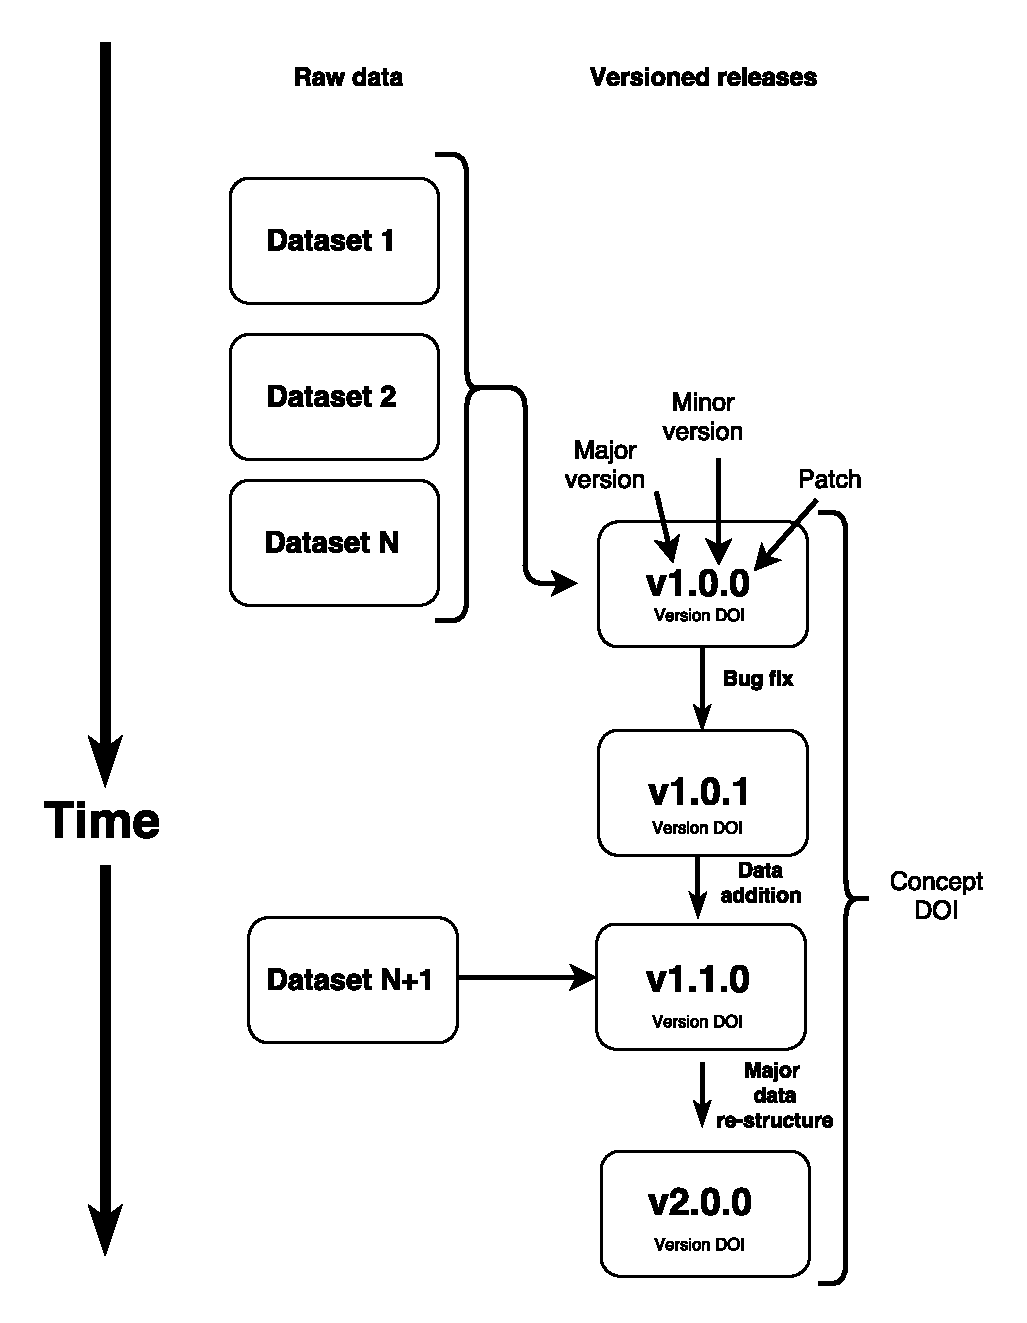
\includegraphics[width=\linewidth]{figures/Figure1.pdf}
\caption{
% could use a more descriptive legend. Maybe walk the reader through it a bit more. Also, I didn’t see (a) and (b) in that figure.
Semantic versioning allows users to anticipate the types of changes that have occurred between successive versions of a dataset.
\textbf{a)} 3 numbers indicate type of change.
\textbf{b)} A typical release stream.}
\label{fig:semantic}
\end{figure}

\newpage


\begin{figure}[!hb]
\centering
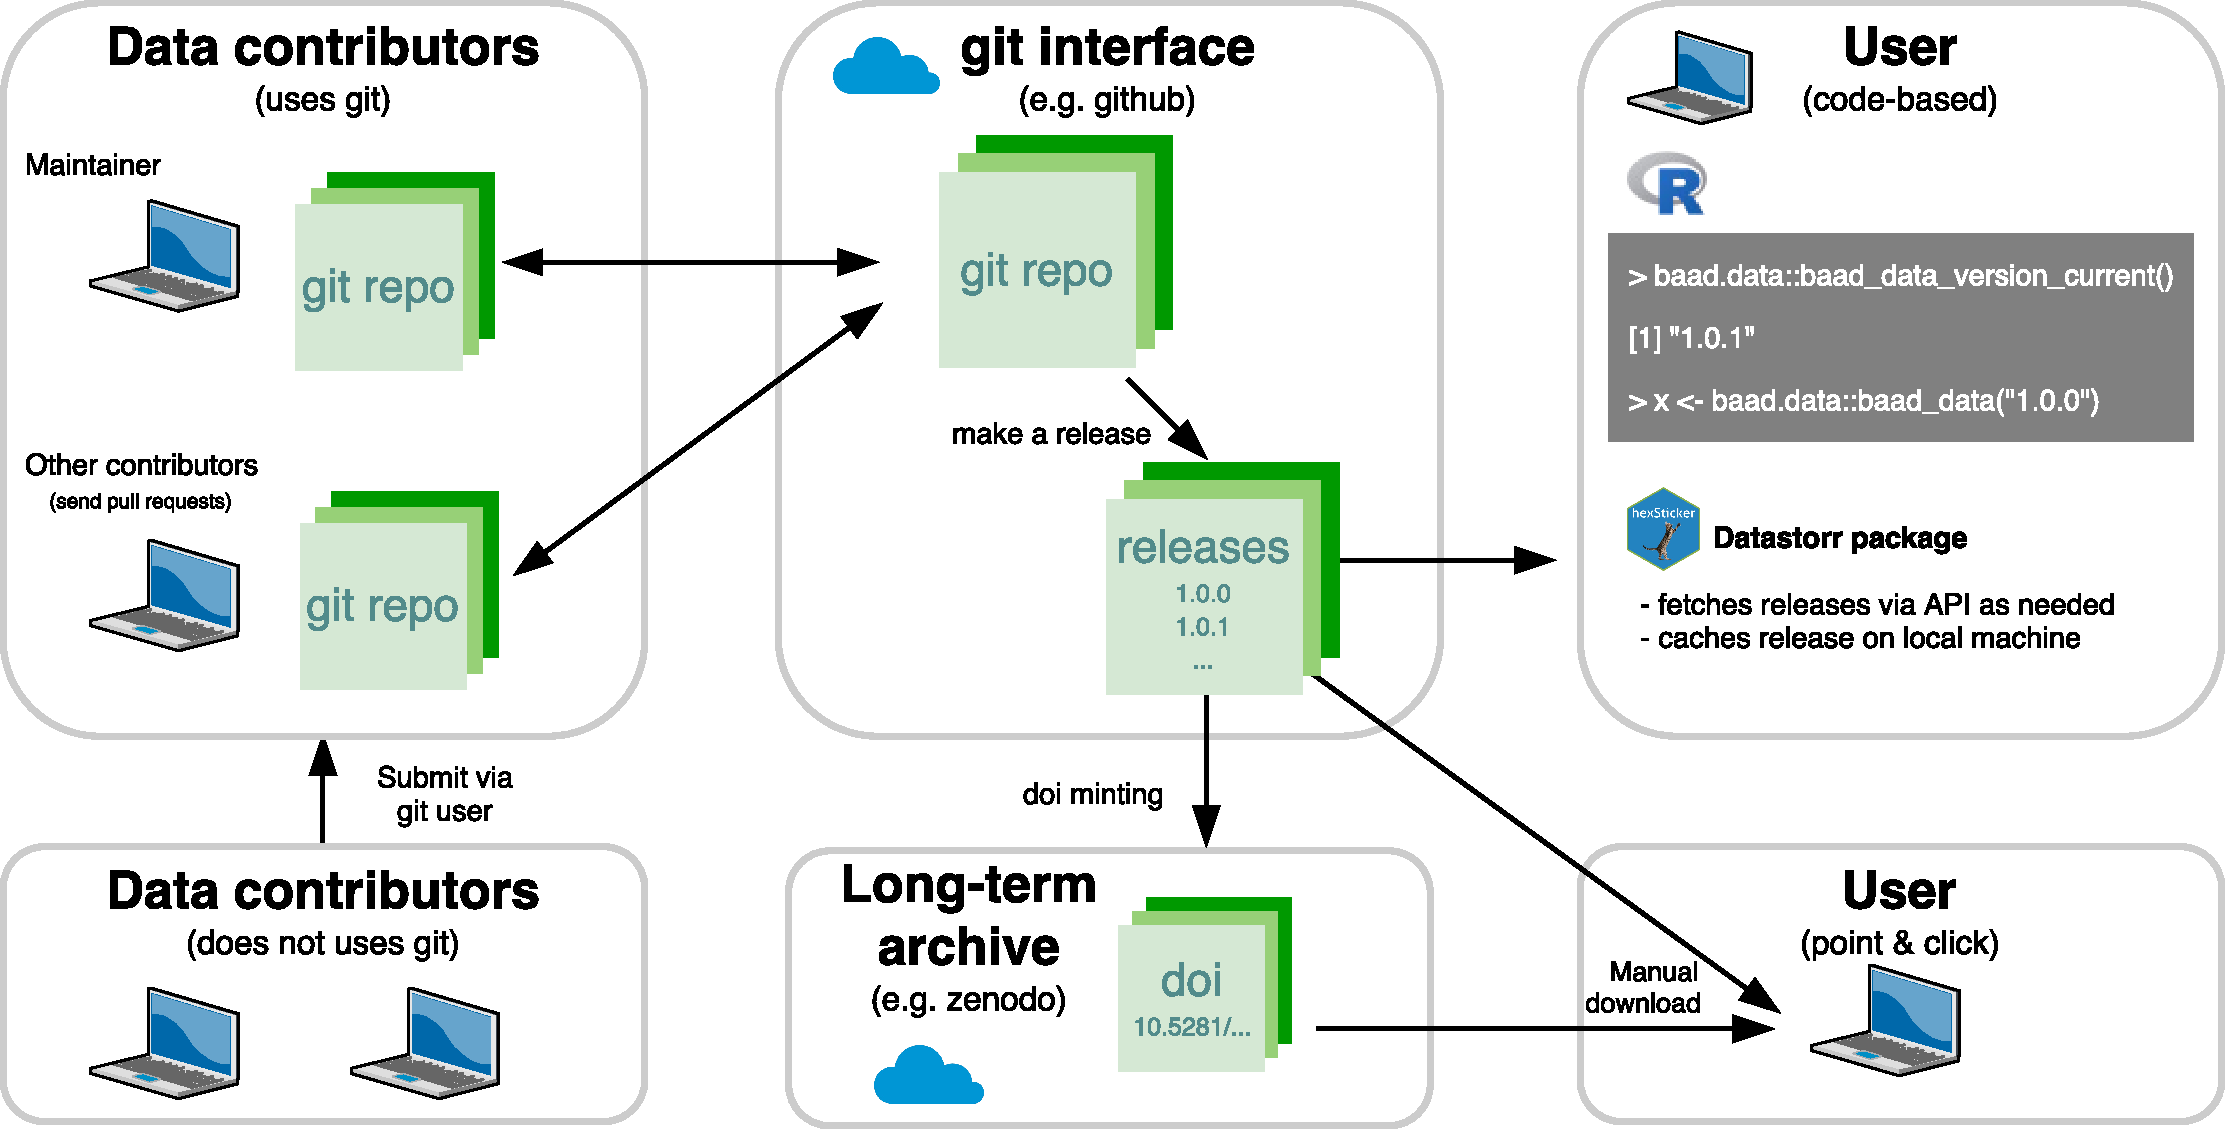
\includegraphics[width=\linewidth]{figures/Figure2.pdf}
\caption{Overview of the different users and technologies involved in distributing a versioned dataset via \texttt{datastorr}.}
\label{fig:technology_stack}
\end{figure}


\bibliography{refs}

\end{document}

